\section{RxJava}
\begin{frame}{Observer to the Rescue!}
	\begin{figure}[h]
		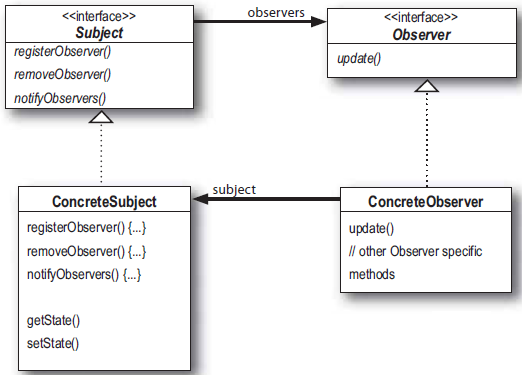
\includegraphics[width=1.0\textwidth,page=1]{gfx/observer_pattern}
	\end{figure}
\end{frame}

\begin{frame}{RxJava Observables}
    \centering
    \begin{tabular}{*3l}
        \toprule
        \textbf{Event} & \textbf{Iterable} & \textbf{Observable} \\
        \midrule
        retrieve data & \texttt{T next()} & \texttt{onNext(T)} \\
        discover error & \texttt{throws Ex.} & \cellcolor{green!50} \texttt{onError(Ex.)} \\
        complete & \texttt{!hasNext()} & \cellcolor{green!50} \texttt{onCompleted()} \\
        \bottomrule
    \end{tabular}
\end{frame}

\begin{frame}{What is RxJava?}
    \centering
    \Large
    \textbf{RxJava's objective is to work on discrete values that are emitted over time (streams), using a push-based architecture.}\\
    \bigskip
    $\rightarrow$ Reactive Programming $\leftarrow$
\end{frame}

\subsection{Streams in Java 8+}\label{sec:java}
\begin{frame}[fragile]{{\nameref{sec:java}}}
  \begin{minted}{java}
List<String> myList =
    Arrays.asList("a1", "a2", "b1", "c2", "c1");

myList
    .stream()
    .filter(s -> s.startsWith("c"))
    .map(String::toUpperCase)
    .sorted()
    .forEach(System.out::println);
  \end{minted}
\end{frame}

\begin{frame}{{\nameref{sec:java}}}
	\begin{itemize}
		\item Pull-based
        \item Single-Use, no forking or reusing
        \item No merging
        \item No time-based operations
	\end{itemize}
\end{frame}

\begin{frame}[fragile]{Back to the [Completable]Future?}
  \begin{minted}{java}
CompletableFuture<String> helloText =
    CompletableFuture.supplyAsync(() -> {
        TimeUnit.SECONDS.sleep(1);
        return "World";
    }).thenApply(name -> {
        return "Hello, " + name + "!";
    }).thenApply(text -> {
        return text + " This is callback chaining!";
    });

System.out.println(helloText.get());
  \end{minted}
\end{frame}

\subsection{Functional Progr.}
\begin{frame}{Functional Programming}
	\begin{itemize}
        \item No side effects
        \item No mutating state
        \item Arbitrary data
	\end{itemize}
\end{frame}

\section{Stream Operators}\label{sec:rxjava}
\begin{frame}{concat()}
	\begin{figure}[h]
		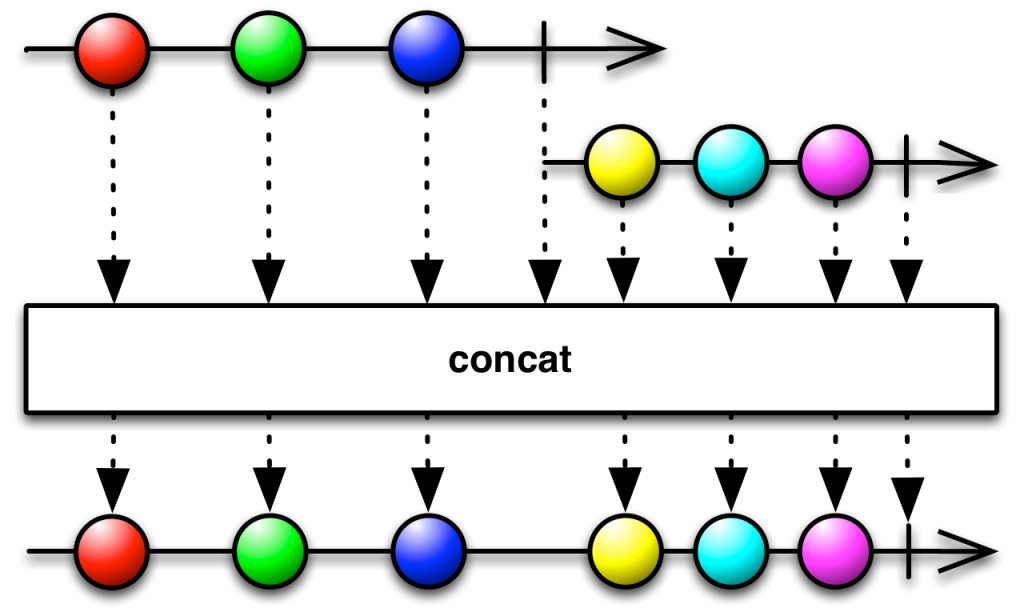
\includegraphics[width=1.0\textwidth,page=1]{gfx/concat}
	\end{figure}
\end{frame}

\begin{frame}{merge()}
	\begin{figure}[h]
		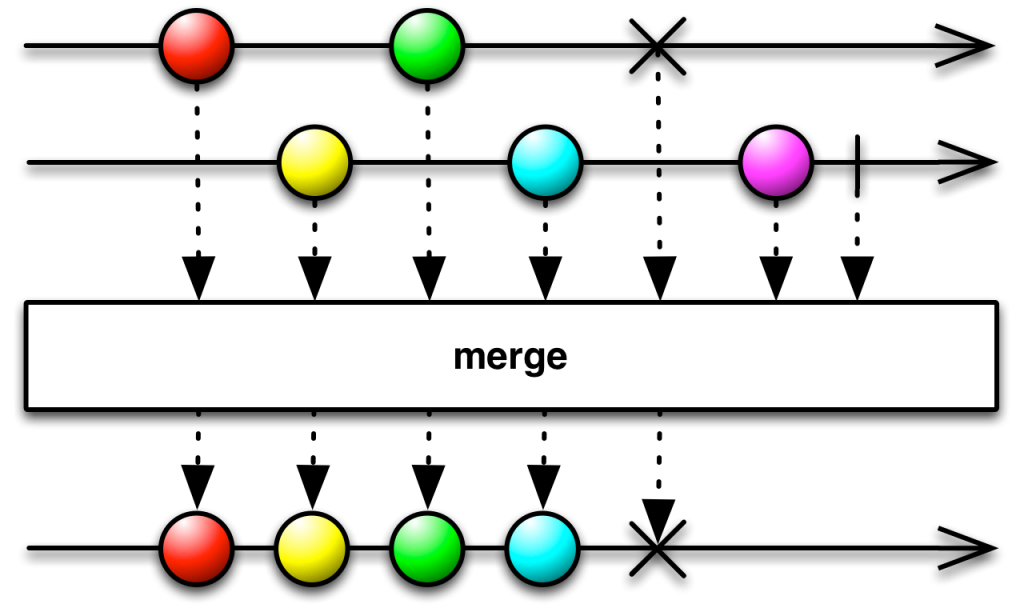
\includegraphics[width=1.0\textwidth,page=1]{gfx/merge}
	\end{figure}
\end{frame}

\begin{frame}{map()}
	\begin{figure}[h]
		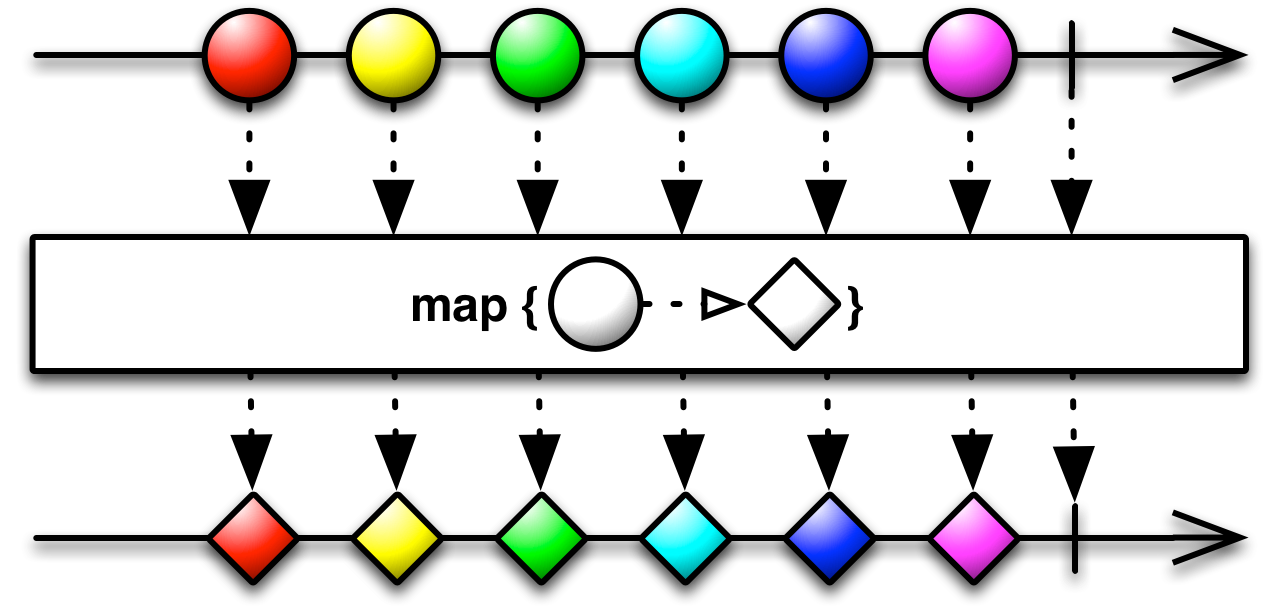
\includegraphics[width=1.0\textwidth,page=1]{gfx/map}
	\end{figure}
\end{frame}

\begin{frame}{filter()}
	\begin{figure}[h]
		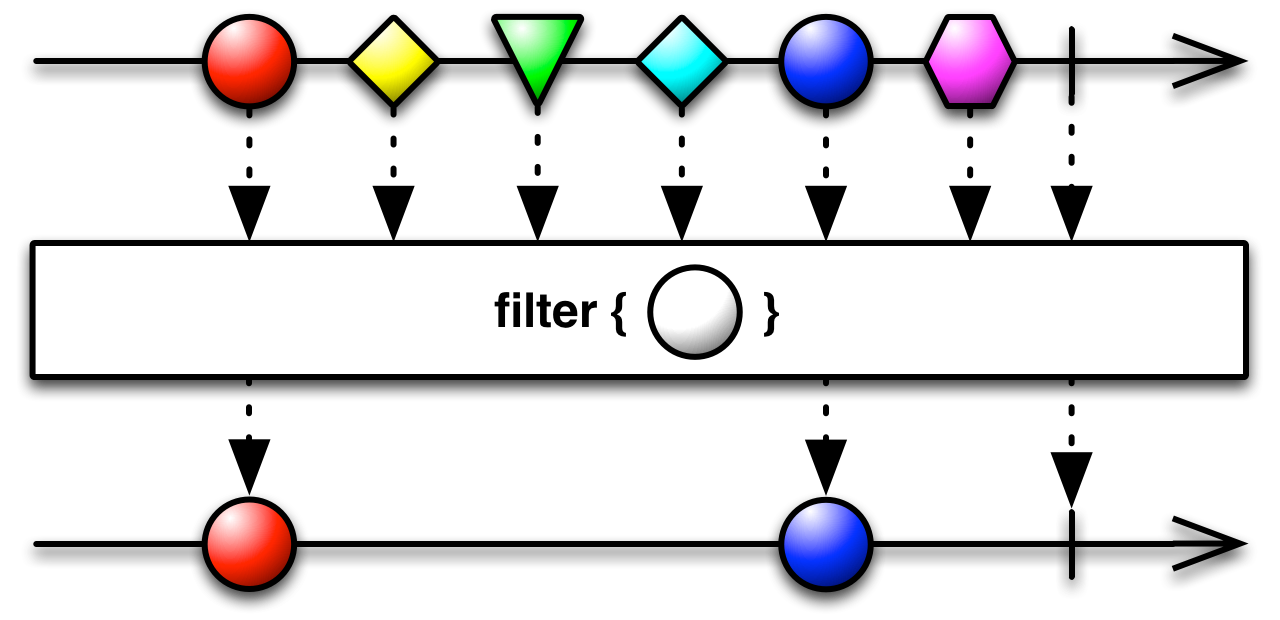
\includegraphics[width=1.0\textwidth,page=1]{gfx/filter}
	\end{figure}
\end{frame}

\begin{frame}{concatMap()}
	\begin{figure}[h]
		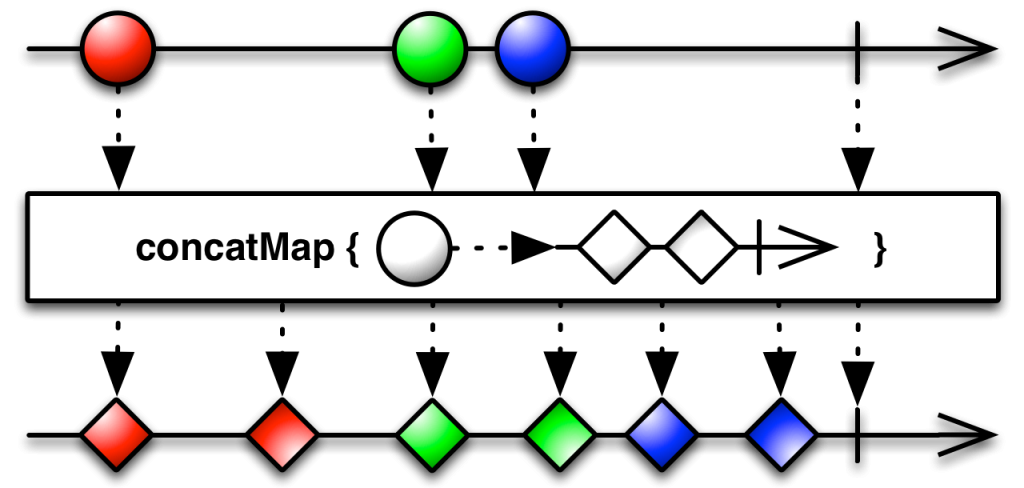
\includegraphics[width=1.0\textwidth,page=1]{gfx/concatMap}
	\end{figure}
\end{frame}

\begin{frame}{flatMap()}
	\begin{figure}[h]
		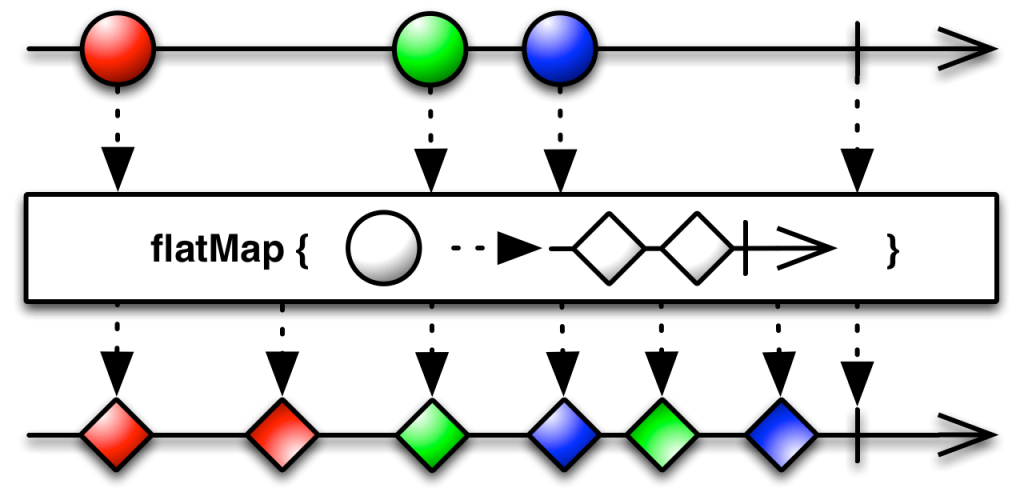
\includegraphics[width=1.0\textwidth,page=1]{gfx/flatMap}
	\end{figure}
\end{frame}

\begin{frame}{reduce()}
	\begin{figure}[h]
		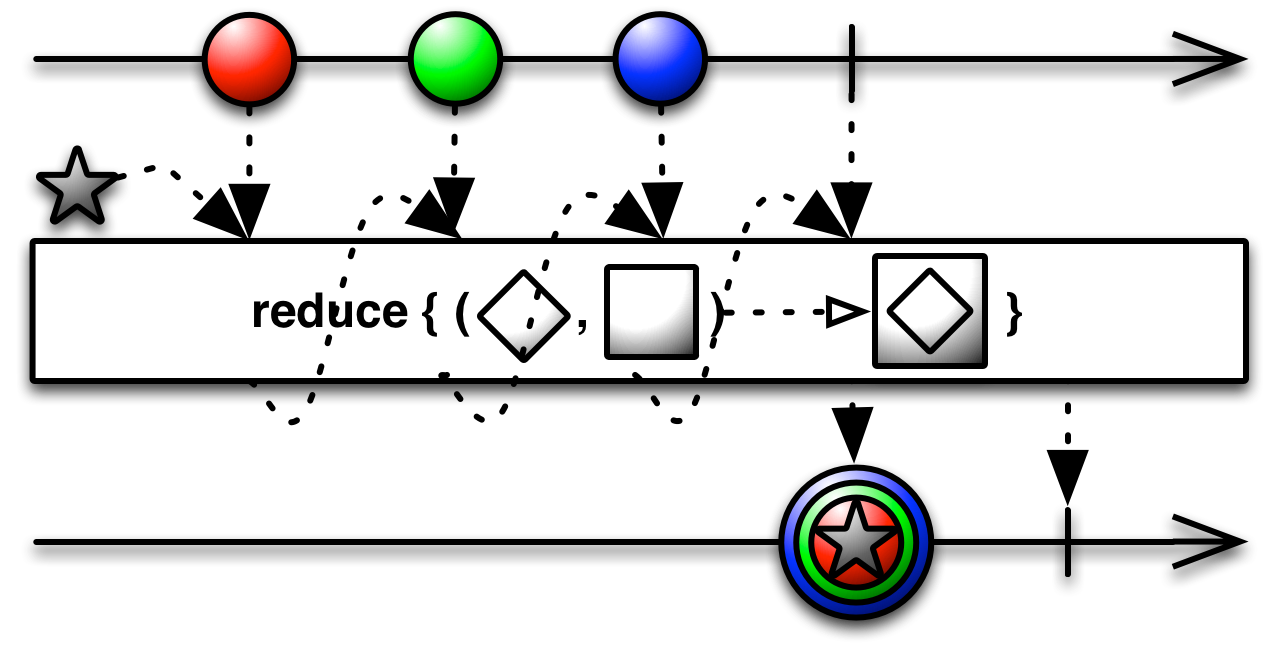
\includegraphics[width=1.0\textwidth,page=1]{gfx/reduce}
	\end{figure}
\end{frame}

\begin{frame}{sum()}
	\begin{figure}[h]
		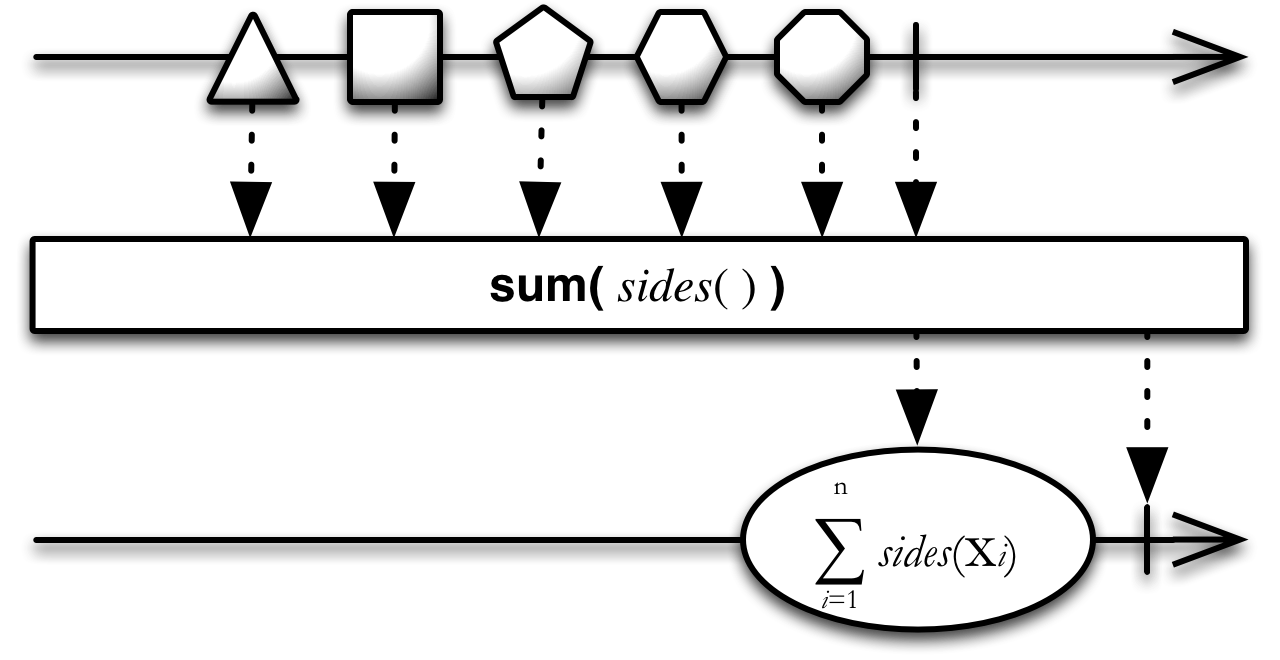
\includegraphics[width=1.0\textwidth,page=1]{gfx/sum}
	\end{figure}
\end{frame}

\begin{frame}{scan()}
	\begin{figure}[h]
		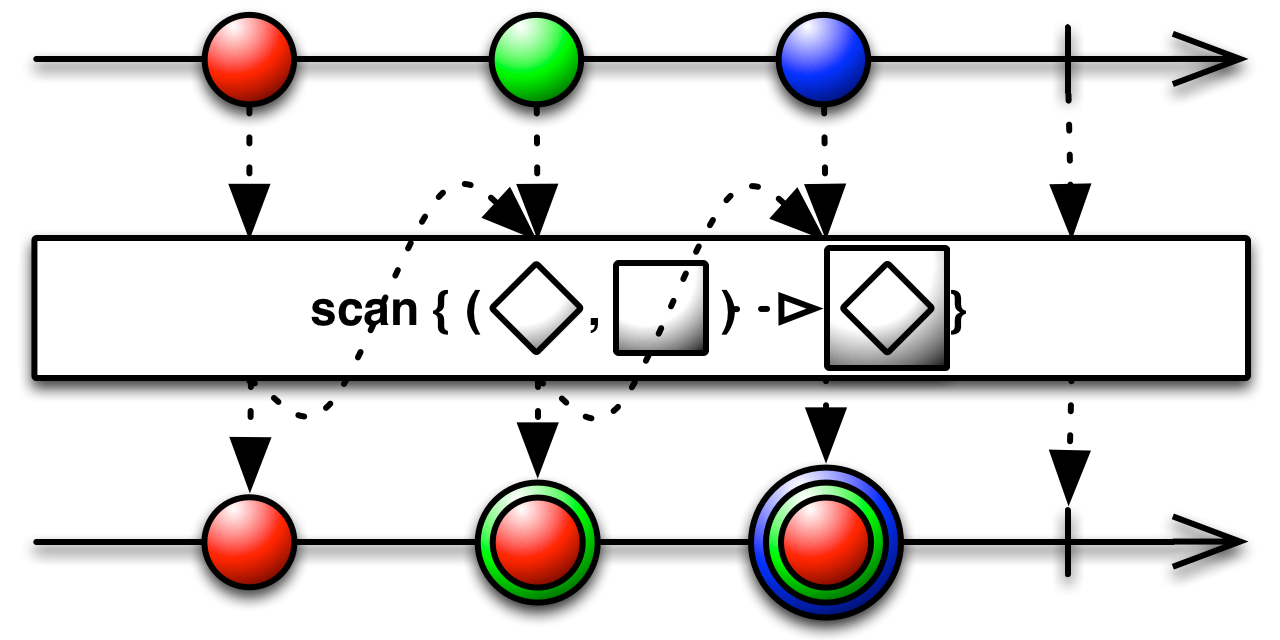
\includegraphics[width=1.0\textwidth,page=1]{gfx/scan}
	\end{figure}
\end{frame}
